% !TeX encoding = UTF-8
% !TeX spellcheck = de_DE

%% Dies gibt Warnungen aus, sollten veraltete LaTeX-Befehle verwendet werden
\RequirePackage[l2tabu, orthodox]{nag}

\documentclass[utf8,biblatex]{lni}
\bibliography{../Dokumentation/Bibliography, ../Dokumentation/snik}

%% Schöne Tabellen mittels \toprule, \midrule, \bottomrule
\usepackage{booktabs}

%% Zu Demonstrationszwecken
\usepackage[math]{blindtext}
\usepackage{mwe}

%% Akronyme
\usepackage{acronym}

%% BibLaTeX-Sonderkonfiguration,
%% falls man schnell eine existierende Bibliographie wiederverwenden will, aber nicht die .bib-Datei händisch anpassen möchte.
%% Bitte \iffalse und \fi entfernen, dann ist diese Konfiguration aktiviert.

\AtEveryBibitem{%
  \ifentrytype{article}{%
  }{%
    \clearfield{doi}%
    \clearfield{issn}%
    \clearfield{url}%
    \clearfield{urldate}%
  }%
  \ifentrytype{inproceedings}{%
  }{%
    \clearfield{doi}%
    \clearfield{issn}%
    \clearfield{url}%
    \clearfield{urldate}%
  }%
}

\begin{document}
%%% Mehrere Autoren werden durch \and voneinander getrennt.
%%% Die Fußnote enthält die Adresse sowie eine E-Mail-Adresse.
%%% Das optionale Argument (sofern angegeben) wird für die Kopfzeile verwendet.
\title[Question Answering auf SNIK]{Question Answering auf einer Ontologie des Informationsmanagements im Krankenhaus}
%%%\subtitle{Untertitel / Subtitle} % falls benötigt
\author[Hannes R. Brunsch]% \and Konrad Höffner]
{Hannes R. Brunsch\footnote{Wilhelm-Ostwald-Schule, Gymnasium der Stadt Leipzig, Willi-Bredel-Straße 15, 04279 Leipzig, Deutschland \email{hrbrunsch@gmail.com}}}
%\and  Konrad Höffner\footnote{Universität Leipzig, Institut für Medizinische Informatik, Statistik und Epidemiologie, Härtelstraße 16--18, 04107 Leipzig, Deutsche \email{konrad.hoeffner@uni-leipzig.de}}}
\startpage{11} % Beginn der Seitenzählung für diesen Beitrag
\editor{Gesellschaft für Informatik}    % Namen der Herausgeber
\booktitle{Studierendenkonferenz Informatik} % Name des Tagungsband; optional Kurztitel
\yearofpublication{2023}
%%%\lnidoi{18.18420/provided-by-editor-02} % Falls bekannt
\maketitle

\begin{abstract}
Mit der beständig fortschreitenden Digitalisierung im Gesundheitswesen wird es immer wichtiger, auch das Wissen über das Informationsmanagement,
also die Verarbeitung von Informationen und die dazu nötigen Schritte u.v.a.m. dort digital und strukturiert erreichbar zu machen.
Diese Arbeit beschäftigt sich mit der vom IMISE entwickelten Wissensbasis SNIK.
Diese enthält Wissen aus dem Bereich des Informationsmanagements im Krankenhaus und soll künftig auch bei dem Studium der Medizininformatik helfen.
Das Wissen soll mittels geschriebener natürlicher Sprache durchsuchbar sein.
Eine Möglichkeit hierfür ist Question Answering.
Es soll möglich sein, dass ein Nutzer eine englische Frage in Satzform stellt und darauf eine Antwort bekommt.
Hierfür gibt es verschiedene Systeme, viele sind allerdings auf andere Wissensbasen spezialisiert.
Das Ziel dieser Arbeit war, nach Systemen zum Question Answering zu recherchieren und letztendlich eines auf SNIK anzuwenden.
Die Antworten wurden außerdem anhand eines vorher definierten Fragenkataloges auf ihre Genauigkeit hin überprüft und bewertet.
Als Kandidat wird QAnswer vorgeschlagen.  
\end{abstract}

\begin{keywords}
Semantic Web \and Question Answering \and Knowledge Graph Question Answering \and Closed Domain Question Answering \and SNIK
\end{keywords}

%\begin{acronym}[nogroupskip]
% fix crazy line spacing
\setlength{\parskip}{0ex}
\setlength{\itemsep}{1.5ex}
% A
\acro{afb}[AFB]{Anforderungsbereich}
\acro{api}[API]{Application Programming Interface}
\acroplural{api}[APIs]{Application Programming Interfaces}
% B
\acro{bert}[BERT]{Bidirectional Encoder Representations from Transformers}
\acro{boa}[BOA]{Bootstrapping linked data}
% C
\acro{cdqa}[CDQA]{Closed-Domain Question Answering}
\acro{cnn}[CNN]{Convolutional Neural Network}
\acroplural{cnn}[CNNs]{Convolutional Neural Networks}
% D
\acro{dag}[DAG]{Directed Acyclical Graph}
\acro{dnn}[DNN]{Deep Neural Network}
\acroplural{dnn}[DNNs]{Deep Neural Networks}
% E
\acro{elmo}[ELMo]{Embeddings from Language Models}
% F
\acro{fsl}[FSL]{Few-Shot Learning}
% G
\acro{gru}[GRU]{Gated Research Unit}
% H
\acro{html}[HTML]{Hypertext Markup Language}
\acro{http}[HTTP]{Hypertext Transfer Protocol}
% I
\acro{imise}[IMISE]{Institut für Medizinische Informatik, Statistik und Epidemiologie}
\acro{iri}[IRI]{Internationalized Resorce Identifier}
\acroplural{iri}[IRIs]{Internationalized Resorce Identifiers}
% J
\acro{json}[JSON]{JavaScript Object Notation}
% K
\acro{kbqa}[KBQA]{Knowledgebase Question Answering}
% L
\acro{lstm}[LSTM]{Long short-term memory}
% M
\acro{mlm}[MLM]{Masked Language Model}
% N
\acro{nlp}[NLP]{Natural Language Processing}
\acro{nlu}[NLU]{Natural Language Understanding}
\acro{nn}[NN]{Neural Network}
\acroplural{nn}[NNs]{Neural Networks}
\acro{nqs}[NQS]{Normalized Query Structure}
% O
\acro{odqa}[ODQA]{Open-Domain Question Answering}
\acro{owl}[OWL]{Web Ontology Language}
% P
\acro{pos}[POS]{Part-Of-Speech}
% Q
\acro{qald}[QALD]{Question Answering over Linked Data}
% R
\acro{rdf}[RDF]{Resource Development Framework}
\acro{rest}[REST]{Representational State Transfer}
\acro{rnn}[RNN]{Recurrent Neural Network}
\acroplural{rnn}[RNNs]{Recurrent Neural Networks}
% S
\acro{snik}[SNIK]{Semantisches Netz des Informationsmanagements im Krankenhaus}
\acro{sparql}[SPARQL]{SPARQL Protocol and RDF Query Language}
% T
\acro{turtle}[Turtle]{Terse RDF Triple Language}
% U
\acro{uri}[URI]{Uniform Resource Identifier}
\acroplural{uri}[URIs]{Uniform Resource Identifiers}
\acro{url}[URL]{Uniform Resource Locator}
\acroplural{url}[URLs]{Uniform Resource Locators}
% V
% W
\acro{w3c}[W3C]{World Wide Web Consortium}
\acro{www}[WWW]{World Wide Web}
% X
\acro{xml}[XML]{Extensible Markup Language}
% Y
% Z
\acro{zsl}[ZSL]{Zero-Shot Learning}
\end{acronym}
%\acused{URL}% Has its own paragraph in the preliminaries.
%\acused{snik}% Explained in Related Work, but appears in Introduction & Preliminaries


\section{Einleitung}

Das semantische Netz des Informationsmanagements im Krankenhaus (SNIK) ist eine
die Domäne des Informationsmanagements im Krankenhaus betreffende Ontologie \cite{domaene}.
Sie behandelt Wissen über Krankenhausinformationssysteme und deren Management.
Dieses wurde aus drei Lehrbüchern \cite{bb,ob,he} und einem Interview \cite{ciosurvey} manuell extrahiert und in RDF modelliert.

Momentan müssen Studierende der Medizininformatik, die nach Wissen suchen, auf eine der drei oben genannten Optionen zurückgreifen.
Jede dieser Möglichkeiten hat jedoch große Nachteile.
Der Resource Description Format (RDF)-Browser gibt nur ein sehr beschränktes Ergebnis aus, und serialisiertes RDF selbst zu lesen ist schwer und unpraktisch.
Die Graphvisualisierung kann im Zweifel unübersichtlich oder überwältigend sein, da es schwer sein kann, überhaupt die Ressource zu finden, zu der man eine Frage hat, und dann zur Antwort zu navigieren.
Im Fall von SPARQL Protocol and RDF Query Language (SPARQL) gibt es einen erheblichen Zeitaufwand für die Studierenden, da sie sich dort erst in die Syntax der Abfragesprache und das Vokabular des Fachbereichs einarbeiten müssen.

Daraus ergibt sich das Problem, dass keine der momentan existierenden Lösungen intuitiv genug funktioniert, als dass es nahezu keine Einarbeitungszeit gibt.
Die existierenden Lösungen liefern zudem nicht übersichtlich ausreichend Informationen, ihrer Expressivität sind demnach deutliche Grenzen gesetzt.

Obwohl ein Ansatz für die Lösung dieses Problems besteht, Question Answering (QA), wirft dieser direkt ein neues Problem für die entwickelnden Personen auf.
Die Implementierung eines QA-Systems mit adäquater Qualität der Antworten ist wesentlich aufwändiger~\citep[S.~3]{qanswer}, als es in einem angemessenem Zeitraum bei stark beschränkten Mitteln möglich ist.

Das Wissen zum Informationsmanagement im Krankenhaus ist komplex und oft nur schwer greifbar.
Es liegt in Form von Lehrbüchern, aber auch in \acs{snik} vor.

Studierende haben selten Zeit, sich ganze Kapitel oder gar Bücher durchzulesen, verfügen jedoch auch nicht über die Kenntnisse SNIK effektiv zu verwenden.
Als Folge müssen sie bei Fragen oft ihren Professor oder andere Studierende hinzuziehen.
Es wäre ungemein einfacher, wenn sie das strukturierte Wissen in natürlicher Sprache abfragen könnten.
QA-Systeme sind im Idealfall 24 Stunden am Tag und 7 Tage die Woche leicht erreichbar und können sofort antworten. 
Besonders in Zeiten während und nach der Covid-19-Pandemie und immer mehr remote work, in denen direkte Kontakte mit Studierenden und Professoren oft eingeschränkt werden müssen und es digitale Veranstaltungen ohne örtliche Präsenz gibt, ist solch ein Werkzeug sehr hilfreich.

\section{Grundlagen}

\subsection{SNIK}

Die in RDF modellierten Quellen SNIKs werden alle in je einer Ontologie abgebildet.
Teilontologien werden mittels der Metaontologie modelliert und miteinander verbunden.
Deshalb ist SNIK sowohl eine Wissensbasis als auch Ontologie:
Es werden zwar keine einzelnen Krankenhäuser abgebildet, aber das Wissen aus verschiedenen Lehrbüchern, die im allgemeinen davon handeln.
Es gibt also mehrere Abstraktionsebenen.
Dadurch ist SNIK eine Ontologie mit Charakteristiken einer Wissensbasis.
Es werden zwar keine wirklichen Individuen abgebildet
- das Wissen liegt immer noch abstrakt aus Lehrbüchern vor, keine speziellen Krankenhäuser und ihre bestimmten Elemente werden betrachtet -
jedoch gibt die Metaontologie allem eine einer Wissensbasis ähnliche Struktur.

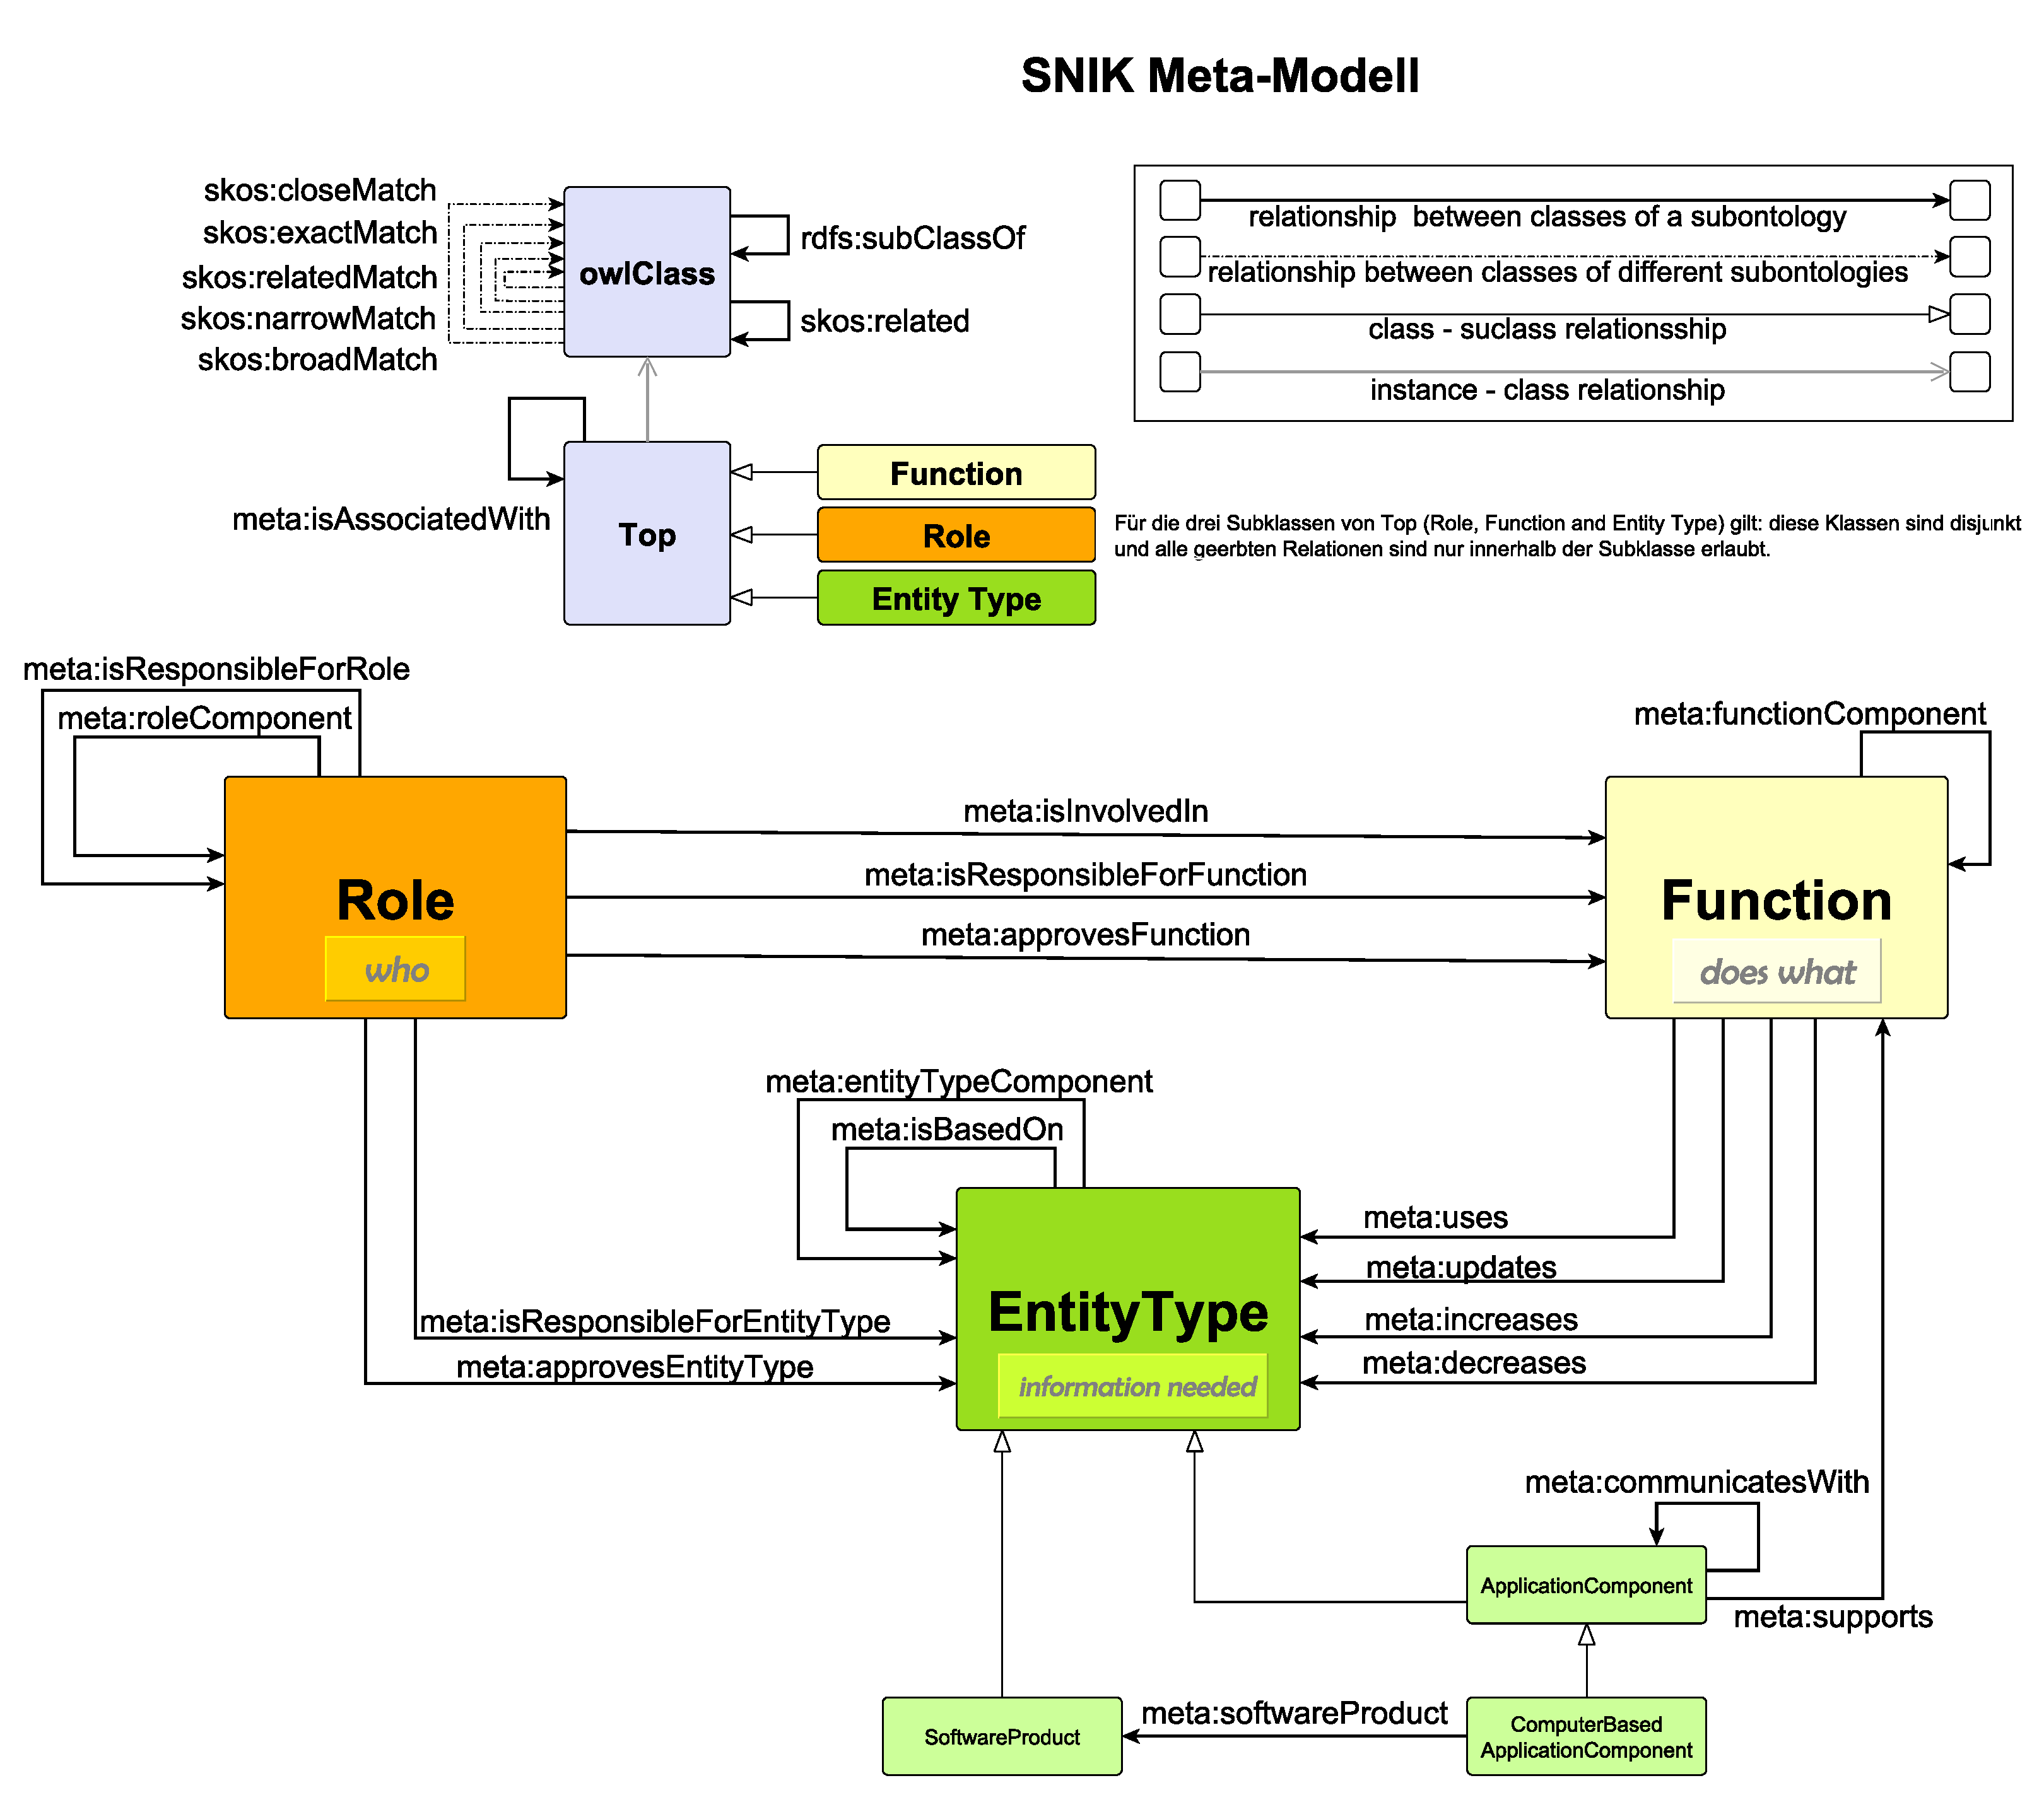
\includegraphics[width=\linewidth]{../Dokumentation/Images/snik-metamodel.pdf}\label{fig:snik-metamodel}

In \cref{fig:snik-metamodel} ist die Metaontologie dargestellt.
Von den drei Klassen \emph{Role}, \emph{EntityType} und \emph{Function} stammen alle anderen Klassen der Teilontologien ab.
Sie beschreiben Personen, Prozesse und Informationen im Krankenhaus.
Alle in der Ontologie vorhandenen Prädikate sind in der Metaontologie definiert.
So sind zwischen den in verschiedenen Teilontologien ähnliche Ressourcen in Relation gesetzt und die Beziehungen zwischen Ressourcen in den einzelnen Teilontologien dargestellt.

\begin{itemize}
%  \item SNIK Metamodell --> Snik ist Ontologie und Wissensbasis in einem, besteht aus Metaontologie und Ontologie, weil Klassen weil Lehrbücher abstraktes Wissen, reden nicht über spezielle Krankenhäuser; Nutzung in QA mittels Verwendung als Wissensbasis und Klassen als Individuen
  \item kurz über QA schreiben, viele Verweise auf QALD etc.
  \item nach neueren Quellen gucken!
  \item Portabilität etc. 
  \item Angeguckte Systeme ein Satz pro System (kleines bisschen mehr über QAnswer KG)
\end{itemize}

\subsection{Question Answering}

\section{Anpasssung von QAnswer KG an SNIK}
\begin{itemize}
  \item Konfiguration: Stopwords, Lexikalisierungen etc.
  \item Verwendung von ausschließlich BB begründen
  \item Materialisierungen und Notwendigkeit derer beschreiben
\end{itemize}

\section{Benchmark}

\section{Ergebnisse}

\begin{itemize}
  \item Training beschreiben
  \item hier die Plots mit den Kurven möglichst auf einer Seite darstellen
  \begin{itemize}
    \item[$\rightarrow$] Mit groupplots \url{https://tex.stackexchange.com/questions/237213/how-to-add-one-single-legend-entry-for-several-plots}
  \end{itemize}
  \item herausfinden wie das offiziell heißt, Lernkurve?
  \begin{itemize}
    \item Die Methodologie dort an sich ist wohl sehr komplex, muss ich wohl auch einen Paragraphen oder so zu schreiben
    \item Paar Ergebnisse, die ich gefunden habe:
    %  \item \url{https://towardsdatascience.com/how-do-you-know-you-have-enough-training-data-ad9b1fd679ee}
    %  \item \url{https://towardsdatascience.com/predicting-the-effect-of-more-training-data-by-using-less-c3dde2f9ae48}
    %  \item \url{https://www.researchgate.net/publication/319272101\_Bootstrapping_the_Out-of-sample\_Predictions\_for\_Efficient\_and\_Accurate\_Cross-Validation}
    %  \item \url{https://www.researchgate.net/post/What\_should\_be\_Optimal\_size\_of\_training\_data}
    %  \item \url{https://machinelearningmastery.com/much-training-data-required-machine-learning/}
    \item Es gibt anscheinend keinen richtigen Namen für den Graphen, würde es also Performance in Abhängigkeit der Datenmenge oder so nennen
    \item Lernkurve ist anscheinend Performance in Abhängigkeit von Zeit, und darauf haben wir nur indirekt und nicht wirklich Einfluss
    \item Die Form scheint recht normal zu sein, also dass das erst recht steil ansteigt und dann einen Grenzwert hat (sieht fast schon wie eine Wurzelfunktion aus bei uns, oder?)
    \item Nur das Ende ist halt komisch, eigentlich scheinen alle zu sagen, dass mehr Daten auch gleich mehr gut sind normalerweise
    \item Liegt also entweder am Training von QAnswer oder an uns, ich würde im Rahmen vom Paper eventuell zumindest nochmal nach Ursachen zu gucken versuchen?
  \end{itemize}
\end{itemize}


\section{Diskussion und Ausblick}

Ein Modell ist immer für einen bestimmten Zweck erstellt und bildet nur einen Teil der Wirklichkeit ab.
SNIK fokussiert sich auf das Beantworten der Fragestellung "Wer (Rolle) macht was (Aufgabe) womit (Objekttyp)?".
Solche Fragen beantwortet das trainierte System auch sehr gut, die größte Herausforderung ist allerdings der "Mismatch" im verwendeten Vokabular eines menschlichen Nutzers zu den Properties der Ontologie.
Während in einer Wissensbasis die Abbildung von Verben zu Properties einfacher ist, weicht besonders bei der Beschreibung von Subklassen und Teil-Ganzes-Beziehungen das Vokabular menschlicher Nutzer oft von den Labels in der Ontologie ab.
Insgesamt erreicht das System bei dieser Art von Fragen  einen F-Score von 0.9... auf ..., siehe ...
Fragen, welche nicht diesem Schema folgen, wie die Leseverständnisfragen aus \cite{bb} (fußnote zu link im zenodo archiv), können selbst nach dem Training nur selten richtig beantwortet werden (F-Score von ... auf ..., siehe ...).
Unserer Einschätzung nach ist dies eine grundlegende Limitierung der gewählten Modellierung, wir erwarten daher auch bei zukünftigen Systemen keine überwiegend richtige Beantwortung der Verständnisfragen.
Wir planen zur Beantwortung allgemeiner Fragen, die über "Wer macht was womit" hinausgehen, das Training von Sprachmodellen direkt auf den Lehrbüchern.
Ein hybrides System aus KBQA und Sprachmodell hat das Potenzial, die Stärken beider Ansätze zu vereinen.

\begin{itemize}
  \item Diskussion von Kurven etc.
\end{itemize}

%% \bibliography{lni-paper-example-de.tex} ist hier nicht erlaubt: biblatex erwartet dies bei der Preambel
%% Starten Sie "biber paper", um eine Biliographie zu erzeugen.
\printbibliography

\end{document}
